% Kopfzeile beim Kapitelanfang:
\fancypagestyle{plain}{
%Kopfzeile links bzw. innen
\fancyhead[L]{\calligra\Large Vorlesung Nr. 16}
%Kopfzeile rechts bzw. außen
\fancyhead[R]{\calligra\Large 03.12.2012}
}
%Kopfzeile links bzw. innen
\fancyhead[L]{\calligra\Large Vorlesung Nr. 16}
%Kopfzeile rechts bzw. außen
\fancyhead[R]{\calligra\Large 03.12.2012}
% **************************************************
\wdh
	Eine Folge komplexer Zahlen $(c_n)n\geq 0$ konvergiert gegen $c \in \C$ wenn gilt:\\
	Für jedes $\e > 0$ gibt es ein $N \in \N$ so dass $n \geq N \Rarr |c_n - c| < \e$\\
	Eine Reihe $\ds\sum_{n=0}^{\infty} c_n$ mit $c_n \in \C$ heißt \ul{absolut} konvergent, wenn die reelle Reihe $\ds\sum_{n=0}^{\infty} |c_n|$ konvergiert.\\
	Absolute Konvergenz \Rarr{} Konvergenz
	Nach 7.15:\\
	Seien $\ds\sum_{n\geq0} c_n = c$ und $\ds\sum_{n\geq0} c'_n = c'$ konvergente komplexe Reihen, mindestens eine absolut konvergent. Dann konvergiert hier Cauchy-Produkt $\ds\sum_{n\geq0} d_n$ mit dem Grenzwert $c \cdot c'$\\
	\ul{Erinnerung:}\\
	$d_n = \ds\sum_{n\geq0} c_k \cdot c_{n - k}$\\
\bew
	Wörtlich wie bei reellen Reihen. \qed
%
% Stefan
% Satz 7.16
%

% Graph für 5)
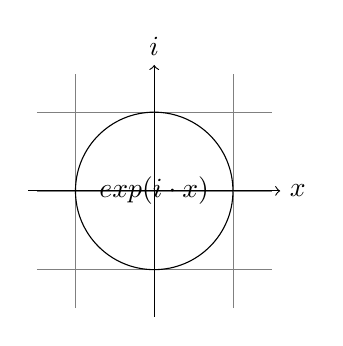
\begin{tikzpicture}[domain=-1.6:1.6]
    \draw[very thin,color=gray] (-1.49,-1.49) grid (1.49,1.49);
    \draw[->] (-1.6,0) -- (1.6,0) node[right] {$x$};
    \draw[->] (0,-1.6) -- (0,1.6) node[above] {$i$};
	\draw (0,0) circle (1cm);
	\node (0.5, 0.5) (expo) {$exp(i \cdot x)$};
\end{tikzpicture}

\uS{Trigonometrische Funktionen}
\sS{Definition}
Sei $x \in \R$\\*
$sin(x) = Im(exp(i \cdot x))$ (Sinus)\\*
$cos(x) = Re(exp(i \cdot x))$ (Cosinus)\\*
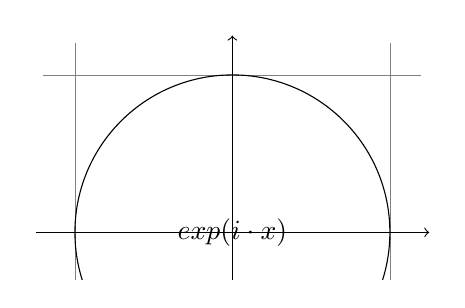
\begin{tikzpicture}[domain=-1.6:1.6, scale=2]
	\clip (-1.3,-0.3) rectangle (1.3,1.3);
    \draw[very thin,color=gray] (-1.2,-0.49) grid (1.2,1.2);
    \draw[->] (-1.25,0) -- (1.25,0) node[right] {$x$};
    \draw[->] (0,-1.25) -- (0,1.25) node[above] {$i$};
	\draw (0,0) circle (1);
	\node (0.5, 0.5) (expo) {$exp(i \cdot x)$};
\end{tikzpicture}
\bem
Für jede komplexe Zahl $z$ gilt $z = Re(z) + i \cdot Im(z)$\\*
\Rarr{} $exp(i \cdot x) = cos(x) + i \cdot sin(x)$ (Eulersche Formel)\\*

%Cos-Graph
\begin{tikzpicture}[domain=-4:4]
    \draw[very thin,color=gray] (-4,-1.25) grid (4,1.25);
    \draw[->] (-4,0) -- (4,0) node[right] {$x$};
    \draw[->] (0,-1.25) -- (0,1.25) node[above] {$i$};
	\draw[color=red] plot[id=cos] function{cos(x)} node[below=3.5cm] {\footnotesize $f(x) = cos(x)$};
\end{tikzpicture}

%Sin-Graph
\begin{tikzpicture}[domain=-4:4]
    \draw[very thin,color=gray] (-4,-1.25) grid (4,1.25);
    \draw[->] (-4,0) -- (4,0) node[right] {$x$};
    \draw[->] (0,-1.25) -- (0,1.25) node[above] {$i$};
	\draw[color=red] plot[id=sin] function{sin(x)} node[below=3.5cm] {\footnotesize $f_1(x) =sin(x)$};
\end{tikzpicture}

\bem
	Die Gleichung $$cos(x)^2 + sin(x)^2 = 1$$
	impliziert $0 \leq cos(x)^2 \leq 1$, $0 \leq sin(x)^2 \leq 1$ somit $-1 \leq cos(x) \leq 1$, $-1 \leq sin(x) \leq 1$.

\sS{Definition}
	\begin{enumerate}
	\item{Eine Abbildung $f: \C \to \c$ heißt stetig in $z \in \C$ wenn gilt:\\*
	Für jedes $\e > 0$ gibt es ein $\delta > 0$ so dass für jedes $w \in \C$ mit $|z - w| < \delta$ ist $|f(z) - f(w)| < \e$}
	\item{$f: \C \to \C$ heißt \ul{stetig}, wenn $f$ in jedem $z \in \C$ stetig ist.}
	\end{enumerate}
	
	% Stefan
	
\sS{Satz}
	Die Funktionen $sin: \R \to \R$ und $cos: \R \to \R$ sind stetig.\\
\bew
Mittels Folgenstetigkeit.\\
Sei $x_n \to x$ mit $x_n \in \R,\ x \in \R$\\*
$\Rarr i \cdot x_n \to i \cdot x$ in $\C$\\*
$\underset{{\footnotesize 7.23}}{\Rarr} exp(i \cdot x_n) \to exp(i \cdot x)$\\*
d.h. $cos(x_n) + i \cdot sin(x_n) \to cos(x_n) + i \cdot sin(x_n)$\\*
$\equ cos(x_n) \to cos(x)$ und $sin(x_n) \to sin(x)$\\*
Somit sind $sin$ und $cos$ stetig in $x$ also stetig.